\subsection{UV-Lampe}\label{sec:UV-Lampe}
Da der Satellit später näher an der Sonne ist und somit höherer UV-Strahlung ausgesetzt ist, wird sich in der Testkammer eine UV-Lampe befinden. Mit dieser UV-Lampe sollen die Effekte der ultravioletten Strahlung auf den Satelliten getestet werden.\\
\vspace{2mm}
Es gibt verschiedene Arten von UV-Strahlung: 
\begin{itemize}
    \item UV-A-Strahlung (Wellenlänge von 320 bis 400 nm)
    \item UV-B-Strahlung (Wellenlänge von 280 bis 320 nm)
    \item UV-C-Strahlung (Wellenlänge von 100 bis 280 nm)
\end{itemize}
\vspace{2mm}
UV-A-Strahlung ist der größte Teil der UV-Strahlung, die die Erde erreicht. Sie kann zu Hautalterung und Hautkrebs führen. Die UV-B-Strahlung wird fast vollständig durch die Ozonschicht absorbiert. Wenn diese Strahlen doch auf die Erdoberfläche treffen, kann es zu Sonnenbrand und Hautkrebs führen. Die UV-C-Strahlung wird vollständig absorbiert und trifft nicht auf die Erdoberfläche. Sie kann künstlich mit Hilfe einer UV-Lampe erzeugt werden. Diese Strahlung wird verwendet zur Desinfektion und Sterilisation.\\
\vspace{3mm}
Die UV-Lampe\autocite{UV-Lampe} in der Testkammer hat eine Wellenlänge von 385 bis 400nm. Diese Art der UV-Strahlung zählt zu der UV-A Klasse und ist am wenigsten schädlich für Menschen. Da der Satellit später in 500 km Höhe sein wird, wäre eventuell eine UV-Lampe der Klasse UV-C besser geeignet. Jedoch ist die Arbeit mit UV-C-Strahlung nicht ungefährlich und kann zu Verbrennungen am Auge und auf der Haut führen.\\
\vspace{4mm}
\begin{figure}[h]
\centering
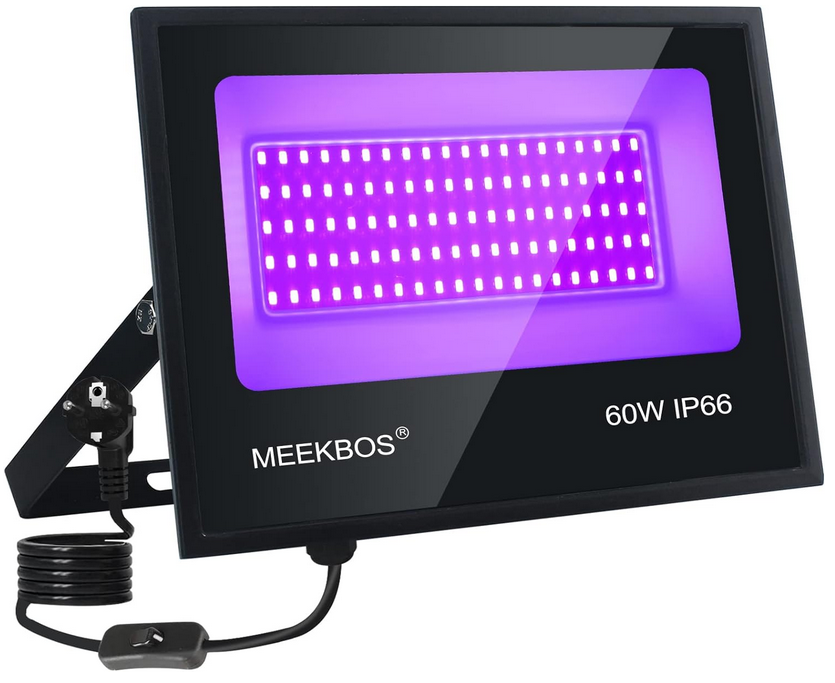
\includegraphics[scale=0.23]{image/uvlampe.png}
\caption{UV-Lampe\autocite{https://m.media-amazon.com/images/I/617AufdHaoL._AC_SL1500_.jpg}}
\end{figure}
\newpage
Die UV-Lampe wird nicht direkt vom \raspi gesteuert. Zwischen dem \raspi und der Lampe ist ein Relais. Dies ermöglicht es, mit einer Spannung von 5V vom \raspi die 230V Netzspannung zu schalten.\\
\vspace{3mm}
\begin{table}[H]
    \centering
    \begin{tabular}{ | c | c | } 
  \hline
   VDD & 5 Volt\\ 
  \hline
   GND & Ground\\ 
  \hline
   Datenleitung (NC) & GPIO18\\ 
  \hline
   Signal (SIG) & GPIO23\\ 
  \hline
\end{tabular}
    \caption{Pinbelegung UV-Lampe}
\end{table}
\vspace{1mm}
Die Programmierung für das Testprogramm befindet sich im Kapitel \ref{sec:Testprogramm UV-Lampe}, und der Programm Abschnitt für die API im Kapitel \ref{sec:Einschalten}
